\documentclass[tikz]{standalone}
\usepackage{tikz}
\usetikzlibrary{positioning, graphs}
\usetikzlibrary{graphs.standard}
\begin{document}
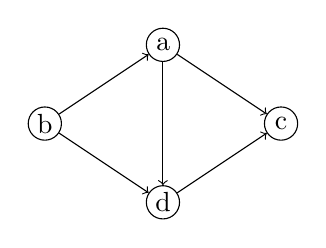
\begin{tikzpicture}
\begin{scope}
		[vertex/.style={draw,circle,inner sep = 0em, minimum size = 1.2em},
		 edgelabel/.style = {fill = white, inner sep = 0.1em, font=\small}]
		\node[vertex] (a) at (0,0) {a};
		\node[vertex] (b) at (-1.5,-1) {b};
		\node[vertex] (c) at (1.5,-1) {c};
		\node[vertex] (d) at (0,-2) {d};
		
		\draw[->] (b) to (a);
		\draw[->] (b) to (d);
		\draw[->] (a) to (d);
		\draw[->] (a) to (c);
		\draw[->] (d) to (c);
\end{scope}
\end{tikzpicture}
\end{document}